%*******************************************************************************
%****************************** Second Chapter *********************************
%*******************************************************************************

% !TEX root = ../thesis.tex

\chapter{Theoretical Background}\label{chap:socialscience}
As abuse and automated decision making systems for detecting abuse can disproportionately affect some populations over others, often communities that are already disproportionately subject to negative societal biases, this dissertation considers abuse not only as a technical question of how to address abuse, but also a social question of how abuse detection systems exist and affect greater societal contexts.
To fully speak to these issues, it is necessary to have a solid understanding of power and processes of marginalisation.
This chapter introduces the core concepts from social science and science, technology studies (STS), and Critical Race Theory (CRT) that can provide such a foundation. 
Beyond this, this chapter reviews the previous literature that the latter chapters of this dissertation relies on. 
Speaking directly towards online abuse, I discuss work on conceptualising online abuse and hate speech.
I briefly introduce the legal landscape surrounding online abuse and content moderation.
Finally, as I work with data that is potentially sensitive, I provide a brief consideration of ethical concerns around using social media data for research.

% In this chapter, we introduce core concepts from social science that we use in this thesis. These concepts will serve as foundational knowledge for how we understand and contextualise abuse and automated systems for detecting abuse.
% This will serve as foundational knowledge for what we interpret as abusive language and hate speech. Subsequently, a consideration of multiple of these may be necessary to determine if speech is derogatory and will inform our recommended solution for handling such speech. Additionally, we seek to introduce how we will use these concepts in the thesis.

\section{Privilege and Marginalisation}

In a consideration of how automated systems might impact different populations, it is necessary to reflect on the positions of groups in society and how they each group is enfranchised and disenfranchised, that is to consider how different groups are privileged and marginalised.
The question of marginalisation and privilege has been subject to a large amount of attention from a vast number of fields, including computer science \citep{Bender:2021,Dinan:2019,Mitchell:2019}, gender studies \citep{McIntosh:1988,Mohanty:1984}, law \citep{Crenshaw:1989}, critical race theory \citep{Benjamin:2019,Myers:2019}, and science and technology studies \citep{Haraway:1988}.
In this chapter, and in this dissertation, I draw on the knowledge produced in critical race theory, science and technology studies, and computer science.

\subsection{Theoretical underpinnings}

In `Black Reconstruction in America' \citet{Dubois:1935} argues that whiteness in America functions as a `psychological wage' providing poor whites in the nineteenth and early twentieth century social status due to not being Black. Through this distinction, he argues that whiteness offers a wage to poor whites who are similarly exploited by capitalism, offering `compensation' beyond monetary compensations. Further, assigning whiteness a higher value, or an idealised position, relies on the devaluation and marginalisation of blackness and Black existence.

% Here he describes a deliberate effort to segregate poor whites and Blacks to prevent potential class-based alliances between the two to avoid collective action. To create such divisions, efforts were made to distinguish whites along racial lines with an aim to align them with their employers. Although in many ways treated the same and living under the same conditions of poverty, whites came to feel a suporiority over Blacks. Notably, in reference to the social mobility of the white working class, \cite{Dubois:1935} writes
% \begin{citequote}{\cite{Dubois:1935}}
% The successful, well-paid American laboring class formed, because of its property and ideals, a petty bourgeoisie ready always to join capital in exploiting common labor, white and Black, foreign and native.
% \end{citequote}

Topics of marginalisation and privilege have been widely explored and is still an active area of research, for instance, contemporary scholars such as Safiya \citet{Noble:2018} and Ruha \citet{Benjamin:2019} examine how computing technologies continue to find ways of subjugating Black people to white supremacist ideals.
Beyond a technological focus, these concepts have also been explored and expanded on to gender \citep{Beauvoir:1953,Butler:1990,McIntosh:1988}, sexuality \citep{McCready:2004}, religion \citep{Beaman:2003}, the intersection of gender and race \citep{Crenshaw:1989,Voigt:2017}, and other aspects of identity.
\citet{McIntosh:1988} describes in her essay ways in which she is privileged as a white woman in comparison to Black women. Thus she highlights in very specific ways in which whiteness affords privileges and Blackness is marginalised.
Throughout the many examples she list, she oscillates between highlighting larger social structures, such as \textit{`I do not have to educate my children to be aware of systemic racism for their own daily physical protection'} and daily experiences \textit{`If a traffic cop pulls me over or if the IRS audits my tax return, I can be sure I haven't been singled out because of my race'}.
Through this description, she calls to attention how processes of marginalisation and privilege operate in both the micro and macro scale, influencing all aspects of life.
Through highlighting ways in which she is privileged, \citet{McIntosh:1988} also highlights ways in which others are marginalised.
It is thus clear that privilege and marginalisation can be thought of as two sides of the same coin, where one is advantaged, another may be discriminated.
In more concrete and operationalisable terms, the concept of privilege describes how some demographics are not systematically and systemically disadvantaged.
In comparison to marginalised communities, privileged communities receive beneficial treatment due to their distance from marginalised identities.
Many social issues have been explained through the concept of privilege such as gender representations \citep{Butler:1990} and police treatment of Black people in the United States of America \citep{Voigt:2017}.

In recent years, there has been a greater focus on social and economic disparities in context of race and gender, including not being financially punished for ones gender expression \citep{Lombardi:2002}; and the increased risk of lethal encounters with law enforcement depending on racial identity \citep{Zack:2015}.

As humans we are never confined to a single identity.
In recognition of this, \citet{Crenshaw:1989} analyses three legal cases in the United States in which Black women were discriminated against while Black men and white women were not.
She argues that the discrimination of Black Women face marginalisation across multiple axes as they exist on the intersection of several marginalised groups: namely being Black and being women.
In one of the three cases presented, Hughes et al. v. General Motors, the plaintiffs, alleged that General Motors had engaged in discriminatory practices when they fired them, based on seniority.
Through the trial it was discovered that all black women hired after $1970$ were fired in a round of seniority-based lay-offs. 
The courts found that no discrimination had occurred on the basis of sex, as white women were not fired, thus the discrimination could not be based on gender. 
The court proposed that the case be consolidated with another active case against General Motors on the grounds of racial discrimination. 
However, as the case was brought on the basis of combination of gender and race-based discrimination, the two lawsuits could not be consolidated. 
Thus, the marginalisation of black women could not be identified along racialised or gendered lines individually. 
To expose the marginalisation faced by black women \citet{Crenshaw:1989} theorises an \textit{intersectional} lens.
\citet{Crenshaw:1989} sheds light on the unique forms of discrimination that are rendered invisible by not considering, or refusing to consider as in the cases she discusses, how existing on the intersection of multiple marginalised identities, such as black women, creates forms of marginalisation that are distinct being marginalised along a single axis.

\subsection{Marginalisation through technology}
% \zw{Add about how equality does not provide equal outcomes or experiences as the world outside of the model is inherently unjust.}

While Crenshaw's \citep{Crenshaw:1989} paper was published more than thirty years ago, the underlying consideration of how multiple identities intersect to create new forms of discrimination is still relevant to new technology that is being developed. 
In $2018$, \citet{Kearns:2018} independently realised that when developing algorithms to detect bias in machine learning systems it is possible to create models that are fair on the basis of singular characteristics, such as race or gender but biased towards the combination of characteristics.
They thus propose an algorithm to identify an optimal number of sub-groups to consider for addressing bias in machine learning systems. 
In recognition of \citet{Kearns:2018} and inspired by \citet{Crenshaw:1989}, \citet{Foulds:2019} propose a new measure of the fairness of machine learning systems that takes into account an intersectional nature of marginalisation.

However, the work of \citet{Kearns:2018,Foulds:2019} both operate within the confines of the machine. As \citet{Blodgett:2020} reminds us, the question of what bias and fairness mean is an inherently normative question, for which reason it is imperative that we define our notion of bias.
\citet{Blodgett:2020} recommend that considerations of bias take into account the social hierarchies that exist outside of the realm of modelling, arguing that `work analysing ``bias'' in NLP systems will paint a much fuller picture if it engages with the relevant literature outside of NLP that explores the relationships between language and social hierarchies`.
Thus, computational work cannot be divorced from the social systems that they exist in.

In another line of recent work on how technology can marginalise, \citet{Sweeney:2013} identified how search results from Google were racially biased against names that are frequently used by African Americans.
\citet{Sweeney:2013} found that when searching for names with a higher association with African Americans, advertisements for examining arrest reports were shown at a higher frequency than when searching for names frequently used by white Americans.
Going a step further, \citet{Noble:2018} shows how search engines reinforce racialized and gendered logics and can aid in radicalisation processes in favour of white supremacy.
She argues that search engines do not merely reflect society and frequent search terms, but create their own reality through ranking.

\begin{citequote}{Safiya \citet[p.148]{Noble:2018}}
  Search does not merely present pages but structures knowledge, and the results retrieved in a commercial search engine create their own particular material reality. Ranking is itself information that also reflects the political, social, and cultural values of the society that search engines operate within[...]
\end{citequote}

Moving beyond the world of search engines, \citet{Benjamin:2019} describes how information technology at large reinforce white supremacy by providing disparate outcomes for different racial groups.
\citet{Benjamin:2019} argues technology encodes such discriminatory biases in spite of, and in part due to, its `allure of objectivity'.
She argues that within our global social structure `codes operate within powerful systems of meaning that render some things visible, others invisible, and creates a vast array of distortions and dangers'.
As technology operates within such systems do not require the explicit intent for racism to produce racist outcomes.
In one example, she highlights the identity number system in India produced discriminatory outcomes when their identity number, Aadhar, could not be identified:

\begin{citequote}{Ruha \citet[p. 133]{Benjamin:2019}}
  There are already reports of citizens being denied welfare services, including children unable to receive school lunches when their Aadhaar could not be authenticated. In this way the New Jim Code gives rise to digital untouchables.
\end{citequote}

\citet{Benjamin:2019} argues that this signifies a discriminatory blindness in technology that are in part brought by the makers, who are predominately white and male.
Moreover, she describes a number of other examples ranging from designating black neighbourhoods as incubators for criminality to using NLP to identify the Roman numeral `X' to represent the number ten, resulting in incorrect street names such as `Malcom Ten Boulevard'.
She argues that `No malice needed, no N-word required, just a lack of concern for how the past shapes the present' and that racism'.

Notably, \citet{Benjamin:2019} proposes four dimensions that information technological systems rely on to discriminate, what she refers to as `the new Jim Code'.
The first dimension is the appearance of impartiality, which she argues is not impartial given its embedding in our global social structures. 
The second is personalisation, which relies on the use of stereotyped information to be created.
The third is merit, although systems of merit themselves are subjective and prejudiced as they too operate within our social structures.
Finally, she argues that the fourth arises from `forward-looking enterprises that promises social good', one such instance being machine learning, and as this dissertation argues, abusive language detection technologies.

\section{The `God Trick'}
% \zw{Discuss Haraway}

\begin{citequote}{Donna \citet{Haraway:1988}}
  No one ever accused the God of monotheism of objectivity, only indifference"
\end{citequote}

In her foundational feminist STS work Donna \citet{Haraway:1988} calls to question the notion of objectivity, critically examining science communication through a feminist lens.
She argues that knowledge production is an \textit{active} process, in which we subjectively construct knowledge based on our particular, subjective bodies.
She argues that in science communication an `objective' position is used to describe the object of study.
However, such an `objective' position, like all other positions comes with its own limitations in what things are rendered visible and what is obscured. 
Thus, an `objective' position is no less subjective, as it privileges the point of view of a particular body marked by subjective social and political meanings and possibilities along the lines of race, class, geography, gender etc. 
In contrast to other `subjective' positions, an `objective' position claims omniscience for itself by denying its own particular embodiments. 
Through this denial the `objective' position obscures its own subjective rootedness.
In the `objective' position's denial of the subjectivity of its own body, the objective position elevates itself over other `lesser subjective bodies', thus playing the `God trick' \citep{Haraway:1988}.
Notably, within the frame of the existence of an `objective' body, as \citet{Haraway:1988} argues the `objective' body is that which is held by `unmarked positions of Man and White' \cite[p. 8]{Haraway:1988}.
Subsequently, the `lesser subjective bodies' are those that do not fit within these, that is people of colour and women.

Through its own disembodiment, the position of objectivity claims to be `universal' and free from embodied socio-political meaning and is therefore applicable in all contexts and can be imposed on all other subjective positions \citep{Mohanty:1984}.
From this it follows that embodied positions are mired in a particular, in contrast to `universal', context.
Accepting new knowledge from these specific embodied represents a threat to the claim of omniscience presented by the disembodied `objective' position.
However, as \citet{Haraway:1988} argues, subjectively embodied positions allow for things to made visible, that are otherwise rendered invisible to the `objective' position.
For instance, in the context of labelling uses of the \textit{n-word}, an exclusive focus on its derogatory use would imply an understanding of the word through a disembodied and universalised position, as this universal position is often occupied by the white male body \citep{Haraway:1988}.
Only through an engagement with the particularised experiences and histories of black bodies can the rich cultural meaning that is crafted in African-American communities be revealed and observed \citep{Rahman:2012}.


% \section{Situated knowledge and subjugated data discourses} \zw{Actually write this as previous work instead of what we're going to do}
% Finally, one cannot talk about data in the context of machine learning without considering where it comes from or how the methods applied to it will affect it. We borrow here loosely from \cite{Fraser:1989} and \cite{Spivak}'s notion of the ``subaltern counterpublics'', that is ``parallel discursive arenas where members of subordinated social groups invent counterdiscourse, and Foucault's notion of dominant and subjugated discourses to understand the processes of marginalisation occurring through the use of machine learning models. Similarly, we rely on \cite{Haraway:1988}'s work on ``Situated Knowledge'' to better understand how machine learning methods, and data used in such methods assume a ``view from nowhere'', employing the ``God trick'' allowing for the illusion of objectivity as a result of applying mathematical modelling to data.

\section{Theoretical Approaches to Content Moderation}
In her ground-breaking book `Behind the Screen: Content moderation in the shadows of social media', Sarah T. Roberts~\citeyear{Roberts:2019} defines Commercial Content Moderation (CCM) as professionals who are employed to `evaluate and adjudicate online content generated by users and decide if it can stay up or must be deleted' \citep[p. 1]{Roberts:2019}, in other words, to ``clean'' internet platforms for content is unwanted by the platforms.
Roberts argues, CCMs are often outsourced to call centres in the global south and boutique firms in North America, with a minority work force held in-house by social media companies \citep{Roberts:2019}.
For outsourced workers, the work is frequently poorly paid and has steep psychological costs to the workers undertaking the job of keeping social media companies.
As one interviewee states `Horror movies are ineffective at this point.
I have seen all that stuff in real life' \citep[p. 122]{Roberts:2019}.
Moreover, she argues that large companies reproduce colonial logics by creating special `ecozones' in Manila, developed in part to respond to the needs for `uninterrupted electricity, the capacity for large scale bandwidth for data transfer, and so on' \citep[p. 183]{Roberts:2019}.
In these zones, call centre workers are increasingly given higher targets and smaller workforces \citep[p. 178]{Roberts:2019} due to the increased competition from other companies in other parts of Asia.
Thus, large social media companies establish their own colonies of exploitation in such ecozones where workers' rights are competing with the risk of companies outsourcing to a different company in a different part of Asia.

\zw{Add page numbers to the quotes}
In her work on theories of social pollution, Mary Douglas \citeyear{Douglas:1966} examines how meaning and community are made through the positive reordering of the environment to separate the subjects and objects that belong and those that do not, i.e.
what is not and what is dirt.
She argues that `dirt is the by-product of a systematic ordering and classification of matter, in so far as ordering involves rejecting inappropriate elements' \citep{Douglas:1966}.
Dirt is then not an independent attribute of an object or subject, but a `residual category rejected from our normal scheme of classifications' \citep{Douglas:1966}.
This classification between what is dirt and what is not, practised through rituals and habits that create coherence within communities, helps establish borders between what and who belongs in a group and what does not.
As communities reject the impure, members of the collective, or in fact society, form a shared meaning.
Through these processes of meaning-making the collective can maintain its integrity.
Dirt then becomes something communities avoid in order to prevent the breakdown of meanings.
Thus to \citet{Douglas:1966}, the avoidance and removal of dirt are not negative processes of removal, they are a `positive effort to organize the environment' \citep{Douglas:1966} of the community in which the removals takes place.
Further she argues that we seek to re-order our environment to make it conform to an idea.

As the identification, demarcation, and expulsion of dirt are collective actions, the definitions and understandings of what constitutes dirt is a subjective in nature and meaning can only be attributed within a given system: `no single item is dirty apart from a particular system of classification in which it does not fit' \citep{Douglas:1966}.
Further, in her conceptualisation dirt is an encompassing label for `all events which blur, smudge, contradict or otherwise confuse accepted definitions' \citep{Douglas:1966}.
Dirt is then contextual, and what is dirty in one situation may not be dirty in another.
She exemplifies this through the mundane: food is not necessarily dirty, `but it is dirty to leave cooking utensils in the bedroom' \citep{Douglas:1966}.

Given the contextual nature of dirt, many might imagine that they are unequivocally able to identify dirt, \citet{Douglas:1966} argues that detecting dirt is complex as with the contextual nature of dirt, it follows that there can be no such thing as absolute dirt or clean, as these depend on the subject observing it.
Thus, what is dirt to one might be valuable to another.
Conversely, as \citet{Lepawsky:2019} argues, the positionality of discarding, or cleaning, may result in discarding or maintaining things that are valuable to one, but are harmful to another.
Who then gets to exert such power to determine what stays and what remains becomes a question of differential power relations.
Indeed, \citet{Hall:1997} similarly ties the classification of dirt and the clean to racist logics of social purification:

\begin{citequote}{Stuart \citet[p.3]{Hall:1997}}
  What you do with dirt in the bedroom is you cleanse it, you sweep it out, you restore the order, you police the boundaries, you know the hard and fixed boundaries between what belongs and what doesn't. Inside/outside. Cultured/uncivilised. Barbarous and cultivated, and so on.
\end{citequote}

By investigating the question of power relationships and commercial content moderation \citet{Lepawsky:2019} extends \citet{Douglas:1966} framework into digital spaces, arguing that such work can help us understand online communities as systems that must constitute themselves through removal, for which human and automated content moderation systems act as the filters that allow for such constitution.

In Hall's \citeyear{Hall:1997}, theory of encoding and decoding, it is argued that expressions are written, or encoded, with a specific understanding which may differ when it is interpreted by the reader from one of three positions: dominant, negotiated, or oppositional.
These moments of interpretation create a space for uncertainty and instability.
Where things have been encoded with one meaning, they can be decoded with a different meaning, e.g.
a semi-colon followed by a close parenthesis may be encoded as an indicator of sarcasm, but decoded as either ungrammatical.
Such oppositional reading can give space for subcultural communities, that stabilise their own meaning-making process such that the community understands a semi-colon followed by a close parenthesis as indicating happiness.

In considering \citet{Hall:1997} and \citet{Lepawsky:2019}, the logics of dirt cannot be disconnected from the oppression experienced by marginalised people.
As \citet{Risam:2015} notes toxic `has become cultural code for irritants and pollutants that disrupt our lived experience'.
\citet{Risam:2015} argues that discourses of toxicity are invoked in cultural conversation between hegemonic and marginalised bodies, and are weaponised against marginalised bodies through an engagement in `toxic slippage'.
Toxic slippage denotes when, in response to `toxic' behaviour, users, or this dissertation theorises, computational methods, engage in toxic behavioural patterns.
Camp theory, as \citet{Schaffer:2015} argues, can offer a ``useful mode of reading for \textit{any} field of study marked by questionable binaries''.
As the question of `toxic'/'non-toxic', `abuse'/`non-abuse', and `hate'/`not-hate' provide such questionable binaries between the desired and undesirable, camp theory's focus on re-evaluating a culture's `trash' offers well-established theoretical frame to re-articulating such concepts, complicating the ways in which content ``can blur and transgress and cover in glitter those boundaries between waste and not-waste [...] without pretending that waste has stopped being waste''\citep{Schaffer:2015}.
As camp provides a mode of queering the understanding of waste from the discarded to the celebrated, it can be read as a ``queer way of knowing, one that emphasises reader relations over any inherent meaning of a cultural object'.
A camp reading of content moderation systems and the decisions produced by them, would then centralise the experiences of the marginalised individual faced with consequences of toxic slippage how dirt must apply to them, fortifying the centrality of the subjective positionality of the individual in relation to the subjective positionalities of the content moderation system.

% \subsection{Pseudonymity and Anonymity in Social Media}\label{sec:pseudonymity}
%
% Previous research on anonymity has considered anonymity as a spectrum \citep{Qian:2007,Donath:1999}, going from the completely anonymous to fully named.
% On the other hand, \cite{Nagel:2015} considers anonymity a more complex space, inhabited by pseudonyms, mononyms, stage names, and usernames amongst others.
% Proponents of named social media sites argue that anonymity encourages anti-social behaviour \citep{Galperin:2011}.
% On the other hand \cite{Nagel:2015}, find this argument misunderstands privacy and identity in both online and offline spaces.
% \cite{Nagel:2015} argue that identity is enacted with territorial and contextual boundaries in the offline world, i.e.
% experiences shared with ones family may differ from those shared with friends, boundaries that are removed in the online world as users interact with their entire social circle, in what \cite{Marwick:2011} refer to as context-collapse.
% \cite{Nagel:2015} suggest that the use of pseudo- and anonymity online can function in a similar fashion to the territorial and contextual boundaries found in the offline world.
%
% To examine how anonymity and pseudonymity is constructed and how it influences, \cite{Nagel:2015} and \cite{Nagel:2013} consider identity on Reddit, a social media site with forums in which users, who are hidden usernames (which may or may not bear reference to their real name) can post and vote on content.
% Specifically, the forum \cite{Nagel:2013,Nagel:2015} consider is ``Gonewild'', a forum which describes itself as ``an amateur exhibitionist community'' \citep{Nagel:2015}.
% On Gonewild, users post nude and semi-nude pictures of themselves, however their faces and names are very rarely associated with these posts.
% In fact, the forum offers guidelines for ensuring safety when posting images:
%
% \begin{citequote}{Emily \cite{Nagel:2013}}
% The internet is a public place. You are posting naked pictures of yourself on the internet[$\ldots$] If you want to be as anonymous as possible, take the following precautions.
% 1. Make a throwaway reddit account.
%
% 2. Don't include your face in your photos. If you must, blur or blackout your features.
%
% 3. Take pictures against difficult-to-identify backgrounds. Plain walls or colours work well.
% \end{citequote}
%
% \cite{Nagel:2013} consider the technological and cultural codes that afford anonymity on Gonewild and the risks of posting sensitive information online in an effort to highlight the importance of nuanced understandings of anonymity online. \cite{Nagel:2013} argue that anonymity plays a crucial role in online communication, as a way for users to segment and limit their audience according to what they aim to share, i.e. many users on Gonewild create throwaway accounts to limit the risk of other reddit users undermining their credibility because they posted on Gonewild:
%
% \begin{citequote}{Emily \cite{Nagel:2013}}
% Such attention, when unwanted, can prompt users to disguise themselves on reddit by creating a ``throwaway'' account.
% \end{citequote}
%
% By creating such throwaway, pseudonymous accounts they are afforded the ability to express their sexual selves in while retaining a disconnect with the rest of their online and offline lives without compromising their ability to interact with their audience or face negative repercussions \citep{Nagel:2015}.

% \noindent With the recent implementation of the General Data Protection Regulation, ensuring anonymity has become more strict than with the DPA. For this reason, we will pseudo-anonymize all users by replacing usernames with a hash and placing all user information in encrypted files, on encrypted disks. User information can thus only be obtained with a key and further obtaining the user hash. Due to the impact of the speaker and listener contexts, it is not possible to entirely anonymize the data sets at this point. It is our intention to fully anonymize the data sets at the earliest possible point, and only use user information if no other option is available.

% \subsection{Anonymity}
% The method that allows for most freedom and safety for users is to fully anonymise data collected on social media. However, due to the phrasing of anonymity in the DPA, which states that a user may not be recoverable obtaining full anonymity on social media data sets is impossible should one seek to work on a user level. In some experiments, namely author profiling, it will not be possible to abstract away from the user level initially. For this reason, at an early stage in our research, it will not be possible to anonymise the data sets fully.
%
% It is our intention to fully anonymise our data sets at the earliest possible point, however, this point will not occur until author profiling tools have been built, such that they can be used in subsequent research. In all subsequent research on social media data, a partial anonymisation will be performed prior to obtaining demographic information by using the author profiling tools. Once the demographic information of a user has been obtained a random hashstring will be generated to identify the user and all user information beyond the demographic knowledge will be dropped. For the sake of reproducibility, a key mapping between user ID's and hashstrings will be stored on a different passport protected encrypted device thus ensuring that the requirements of the DPA are fulfilled.


% \subsection{Safety}\label{sec:ethics:safety}
% Given that the topic of thesis may touch upon some very sensitive issues, such as gender and racial biases, it is necessary to ensure the safety of participants and researchers involved. Given that much of the controversial data will be personal data, this safety is largely ensured by following the Data Protection Act (DPA) and the General Data Protection Regulation (GDPR) through their focus on ensuring that un-anonymized participant data is only available to the researchers working on the project. Indeed, the DPA suggests that data is anonymized at the earliest possible step, and that it is stored on encrypted drives such that participant, and in extension researcher safety is ensured.
%
% In this project, there will be a need for retaining un-anonymized data sets in regards to determining the speaker and listener demographics. To ensure participant safety, we will ensure that any data sets that have not been released publicly are stored in encrypted folders, and encrypted devices where possible. In addition, access to the data will be restricted to the active researchers in the project and potentially the respective supervisors.

% \section{Participant Agency and Informed Consent}
% At this point, the requirements of the GDPR for consent in social media research is not entirely clear to us. We will follow the requirements of the GDPR and update this once we have a clear understanding of how and if consent will be required.
% The social media aspects of this project calls for unobtrusive observation on social media, it is not possible to conduct the research while obtaining informed consent from the users. Rather, we approximate consent by publication. Given the public nature of Twitter, which will be our primary if not only source of social media data, we argue that users are aware of their tweets being published to the world, in addition, should users frequently use ``hashtags'', a method for categorising and widening the audience of tweets, it implies that not only are they aware of the public nature of Twitter, they are explicitly seeking to widen the audience of their tweets to a global scope. In our project, we will collect tweets using hashtags and the tweets users of those hashtags publish. In order to ensure that the users are aware and explicitly utilise the public nature of Twitter, we will not use tweets from users that use hashtags less than at a given ratio\footnote{We need to determine this ratio based on real use of Twitter.}
%
% To ensure user agency, we will remove tweets that are deleted and we will only collect tweets from public accounts.

\section{The Legality of Abuse}

As the detection of abuse may be closely linked to the content moderation and the removal of content, any consideration of tools with the purpose of identifying abuse must also consider the legal context context in which they may operate, to situate the work in computational content moderation within the social and political realities that it exists in.
Here, I consider two forms of legal contexts: 1) platform policies and 2) regulatory frameworks and their influences on using automated methods for detecting abusive language.

\subsection{Moderation Practices}
To understand how content moderation can work, it is necessary to consider the communicative power of frameworks for reporting inappropriate content.
\citet{Crawford:2016} argue that reporting mechanisms constitute a communicative channel between users and the platforms.
Thus, the question of content reporting becomes a more nuanced space than the question of what content is permissible, instead it becomes a question of what is desired by different user communities \citep{Crawford:2016}.
Simultaneously, reporting frameworks also allow for companies to control the expressiveness of the communication between users and the company and the volume of this communication \citep{Crawford:2016}.
On one hand the expressiveness of the reporting can be controlled by the level of detail users are afforded when reporting, on the other hand, volume can be controlled through the ease of access to the flagging mechanism.
When platforms set the degree of expressiveness of the flagging mechanism, the detail allowed provides a signal on whether the platform are interested in the particular way content offends or simply that users find that the content should be disallowed \citep{Crawford:2016}.

While often a flagging is often a solitary effort performed by a single user, it can also be the result of a strategic means of communication by a coordinated user group.
For instance, a group of bloggers angered by pro-Muslim content on YouTube started the `Operation Smackdown' campaign in 2007 to remove such content.
In this coordinated attack, coordinating users created lists of YouTube videos for other users to flag as `promotes terrorism' \citep{Crawford:2016}.
Here we also see how flagging campaigns can be used to reinforce social hegemonies.

On the other hand, when platforms remove content that is socially acceptable to a large majority, there are strong backlash against the platforms.
In one such event, Facebook removed an image of two male actors kissing on the television show EastEnders.
Following this removal there was a large outrage, accusing Facebook for perpetuating homophobia while leaving images of straight couples kissing.
Following this controversy, Facebook reversed their decision to remove the image and apologised for the removal \citep{Crawford:2016}.

\subsection{Platform Policies}

Many large social media companies lay out their policies for acceptable behaviour on their platforms, often detailed in their user guidelines. Many of these have similar phrasing on the acceptance of abusive language,\footnote{For the full policies see \url{https://en-gb.facebook.com/communitystandards/hate_speech} for Facebook's policy on hate speech, \url{https://help.twitter.com/en/rules-and-policies/hateful-conduct-policy} for Twitter's policy on hate speech, and \url{https://www.redditinc.com/policies/content-policy} for Reddit's policy on prohibited content.} in \autoref{fig:policies} I show excerpts of the policies on hate speech and prohibited content of three social media platforms.

In all three excerpts of the policies, we see a prohibition of content which attacks others, Reddit's policy on encouraging and inciting violence they further outline that users should not post content that\footnote{for the full policy see \url{https://www.reddithelp.com/en/categories/rules-reporting/account-and-community-restrictions/do-not-post-violent-content}}

\begin{quote}
  [\dots] that encourages, glorifies, incites, or calls for violence or physical harm against an individual or a group of people
\end{quote}

Establishing similar outlines for acceptable conduct as seen on Twitter and Facebook. Facebook note in their Community Standards Enforcement Report\footnote{See report here: \url{https://transparency.facebook.com/community-standards-enforcement\#hate-speech}} that they acted on $4$ million items for hate speech and $2.8$ million items for bullying and harassment in the period of January to March 2019. The report does not detail the number of user reports received, nor the amount of content which was not removed.\footnote{Acted on here means acknowledging that the content does violate community standards yet and an action was taken by Facebook.} Considering the scale of the items which have actions taken for different kinds of abuse, there is an incentive to allow for some automation to guide the attentions of human moderators or decrease the number of items which moderators need to consider.\footnote{The Community Standards Enforcement Report details that automated systems are deployed but do not detail the performances of the system in terms of accuracy, precision, or recall.}

While Facebook report high numbers of removals, the performance of their (human and automated) moderation practices have been the source of criticism as a number of activists have reported being temporarily banned for speaking about racial discrimination while abuse and discrimination received is not addressed \citep{Sharif:2019} and common users noting that simply talking about race may mean that your post is removed, particularly if the poster is not white \citep{Guynn:2019}. A report from Pro Publica details that the policies of Facebook in determining whether a post violates community guidelines, by seeking global standards, effectively ``protect the people who least need it and take it away from those who really need it.''\citep{Angwin:2017}

\begin{figure}[!htb]
  \centering
  \begin{minipage}{0.45\textwidth}
    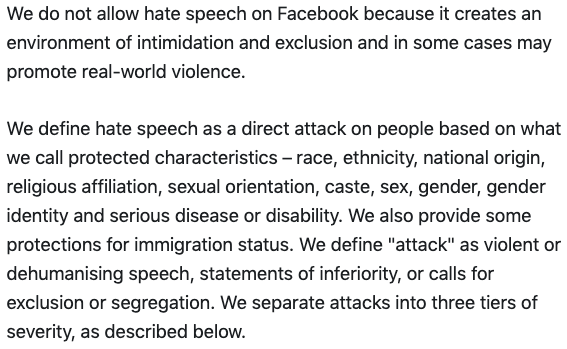
\includegraphics[width=\linewidth]{Chapter2/Figs/Facebook.png}
    \caption*{(a) Facebook}
  \end{minipage}\hfill
  \begin{minipage}{0.45\textwidth}
    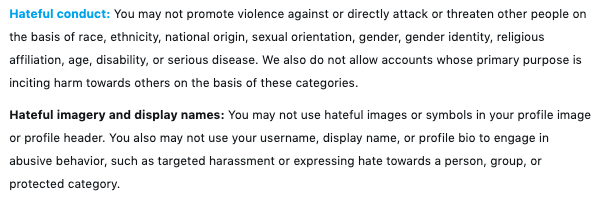
\includegraphics[width=\linewidth]{Chapter2/Figs/Twitter.png}
    \caption*{(b) Twitter}
  \end{minipage}\hfill
\end{figure}
\begin{figure}
  \centering
  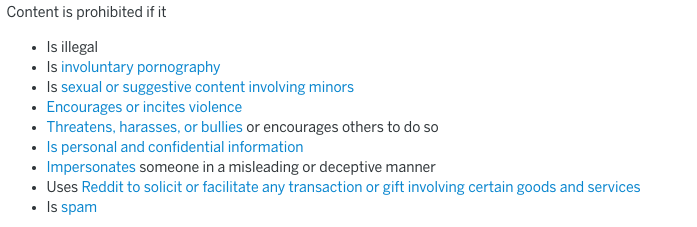
\includegraphics[width=\0.45linewidth]{Chapter2/Figs/Reddit.png}
  \caption*{(c) Reddit}
  \caption{Excerpts of policy on prohibited content and hate speech from Facebook, Twitter, and Reddit.}
  \label{fig:policies}
\end{figure}

Considering how such policies are described, understood, and enacted by commercial content moderators, content moderation algorithms, and users, \citet{Kirtz:2021} perform an analysis of how different platforms describe their community guidelines and their downstream implications for content moderation technologies and user experiences. They argue that the platform policies fail `at the level of policy by mis-communicating , obscuring or sometimes even misleading the public' \citep[p. 5]{Kirtz:2021}. Moreover, due to such failures of policy, \citet{Kirtz:2021} argue that the platforms fault lines are particularly apparent for marginalised communities that are the subject of disproportionate abuse. Subsequently, the data generated user reports which is used to train automated content moderation systems mimic such failures providing little protection along gendered and racialised lines \citep{Kirtz:2021,Waseem:2018}. However, while data provides one source of such errors, modelling techniques also give rise to such failures. For instance, \citet{Kirtz:2021} also identify the use of pre-trained word embeddings as source of propagating such biases, as word embeddings frequently contain biases against marginalised communities \citep{Speer:2017}. \citet{Kirtz:2021} argue that such embedded biases compound any potential biases that policies and content flagging mechanisms introduce.

\subsection{Regulation}
In recent years several different governments have sought to address the issue of online abuse, for instance the British Home Office \citep{HomeOffice:2016} and the European Commission \citep{EUCommission:2016} gave guidelines and a call to action to social media networks.
In a different approach, the German government passed the Network Enforcement Act (NetzDG) \citep{NetzDG:2017} in an aim to provide regulation to curb online abuse and misinformation.
The regulation states that online platforms will face fines if they systematically fail to remove hate speech within $24$ hours.

Building on this, the European Union is currently considering regulation on disseminating terrorist content which may have implications on hate speech and how social media platforms deal with issues such as hate speech \citep{EUCommission:2018} through the difficulty in distinguishing between content which promotes terrorism and content which is simply hateful - a consideration which is highlighted in the response from the European Union Agency for Fundamental Rights (FRA).
In their opinion, the FRA suggest that the proposed regulation should provide a clear definition of terrorist content which limits it to inciting or promoting terrorist activities or providing instructions on the making or use of weapons \citep{FRA:2019}.
A key point of the regulation states that the platforms must remove content within $1$ hour of receiving notice from a trusted authority.

More severely, two bills on sex trafficking were passed in the United States of America, namely the Stop Enabling Sex Traffickers Act (SESTA) and the Fight Online Sex Trafficking Act (FOSTA).
These two bills aim to prevent sex trafficking by removing sexual solicitation online.
While the critiques of the bills are numerous for flaws in their conceptualisations \citep{Romano:2018}, impact on criminal investigative work \citep{Q:2018} and the consequences for sex workers - including missing persons and deaths of sex workers \citep{Blue:2018,Simon:2018}, the implications of the bills are far greater in three aspects:

\begin{enumerate}
  \item{The bills weaken \citep{Romano:2018,Stryker:2018} in Section 230 of the Communications Decency Act (CDA) - which holds that computer service providers are not publishers and thus not liable for content on the platform \citep{EFF:230},}
  \item{the bills are effective retroactively \citep{Stryker:2018}, therefore necessitating moderation of both new and historic content, and}
  \item{the bills do not require a request to remove content prior to potential consequences for not upholding the laws.}
\end{enumerate}

While the weakening of Section 230 of the CDA falls in line with the European and German regulations by holding social media companies accountable for the content on their platforms,\footnote{We note here that the CDA only applies to the legal territories of the United States of America.
Thus, the European regulations have no bearing on the development of the Section 230 of the CDA.} the European and German initiatives are designed such that social media platforms respond to flagging and requests for content removal from authorities.
Furthermore they are not in effect retroactively.
These differences strongly encourage the use of machine learning to be applied without regard to the precision of the systems.

\section{Ethical Considerations}

As this dissertation deals with data that is published by individuals who very often are private citizen, it is necessary to consider different aspects of the ethical use of social media data use.
As I only make use of previously published data, informed consent cannot be obtained directly, as I do not have access to the necessary contact details.
Moreover, several of datasets do not provide the user information to even consider access.
Finally, as many of the datasets are several years old any contact information that could be gleaned from the data sets have, in many cases, decayed.

As informed consent is not sought for the data, the need for a consideration of anonymity and privacy is only heightened, to ensure that private citizens are not exposed additional harms.
All experimental parts of this dissertation have undergone ethics review for risks and harms and been approved for study.
In this dissertation, I exclusively make use of previously published datasets. Some data in these datasets are entirely anonymised, others are entirely de-anonymised, and the remainder exist in this spectrum.
For my experimental work, I exclusively make use of previously published, and currently publicly available, data.
Taking an additional step to prevent harms to the data subjects, I anonymise all data where appropriate.


\section{Summary}
In this chapter, I have introduced several key notions and concepts that will lay a theoretical and philosophical foundation of my work.
Specifically, this chapter introduces the notions of privilege and marginalisation and previous work on how these concepts relate to computational techniques. I further provide a background to theory surrounding content moderation. Finally, I provide a consideration of ethical use of social media for research and conclude the chapter with a brief overview of two legal aspects of abuse.
